% Intended LaTeX compiler: xelatex
\documentclass[10pt, svgnames]{beamer}
\usepackage{graphicx}
\usepackage{longtable}
\usepackage{wrapfig}
\usepackage{rotating}
\usepackage[normalem]{ulem}
\usepackage{amsmath}
\usepackage{amssymb}
\usepackage{capt-of}
\usepackage{hyperref}
\usetheme{metropolis}
\author{Sappinandana Akamphon}
\date{\today}
\title{Material Selection}
\subtitle{ME 310: Mechanical Design}
\usepackage{booktabs}
\usepackage{pgfplots}
\pgfplotsset{compat=1.18}
\institute{Department of Mechanical Engineering, TSE}
\date{}
\usetikzlibrary{patterns,shapes,arrows,decorations}
\AtBeginSection[]{\begin{frame}{Outline}\tableofcontents[currentsection]\end{frame}}
\definecolor{lightblue}{RGB}{180,220,255}
\usetikzlibrary{arrows,calc,decorations,shapes,decorations.pathmorphing,patterns}
\usepackage{multirow}
\usepackage{pgfplots}
\usepackage{array}
\hypersetup{
 pdfauthor={Sappinandana Akamphon},
 pdftitle={Material Selection},
 pdfkeywords={},
 pdfsubject={},
 pdfcreator={Emacs 30.0.50 (Org mode 9.6)}, 
 pdflang={English}}
\begin{document}


\section{Mechanical Springs Overview}
\label{sec:orgdc87a8c}

\begin{frame}[label={sec:org0ae4b8c}]{Mechanical Spring Usage}
\begin{columns}
\begin{column}{0.4\columnwidth}
\begin{itemize}
\item Springs are used for
\item Energy storage
\item Impact absorption
\item Actuator
\end{itemize}
\end{column}

\begin{column}{0.6\columnwidth}
\begin{center}
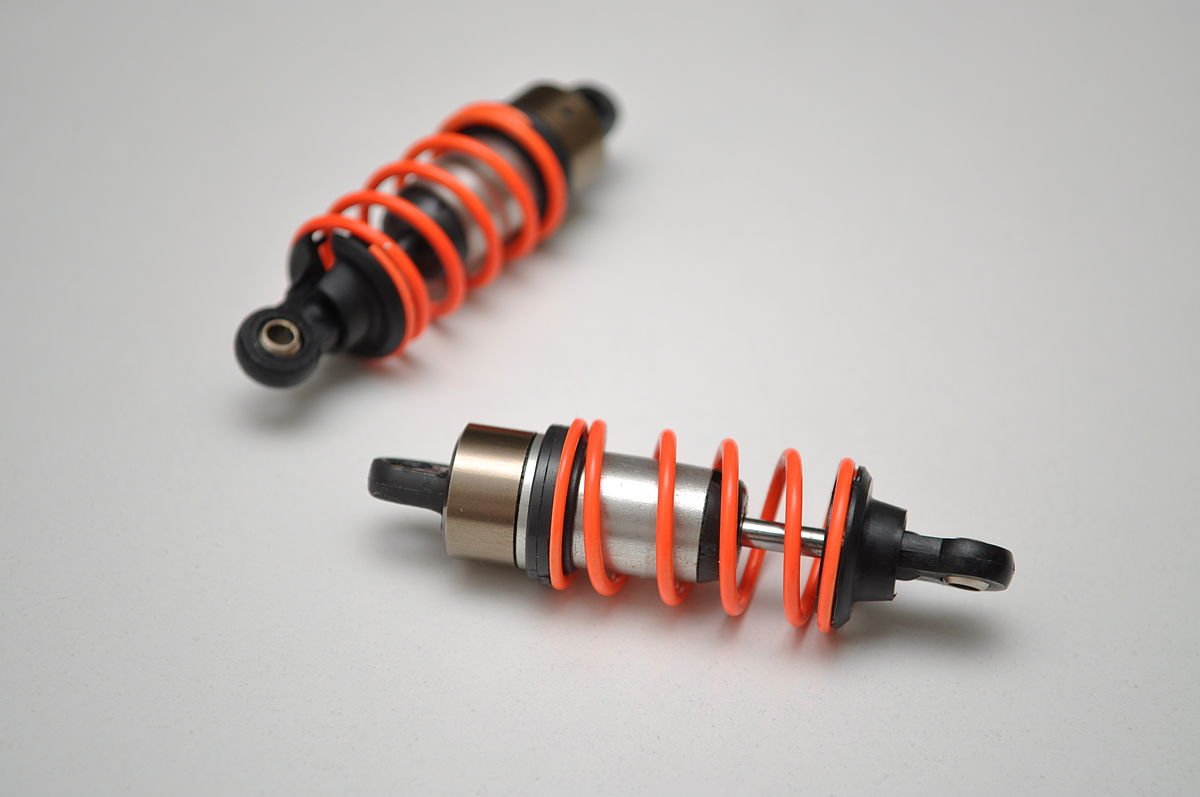
\includegraphics[width=.9\linewidth]{./pictures/shock-absorbers.JPG}
\end{center}
\begin{center}
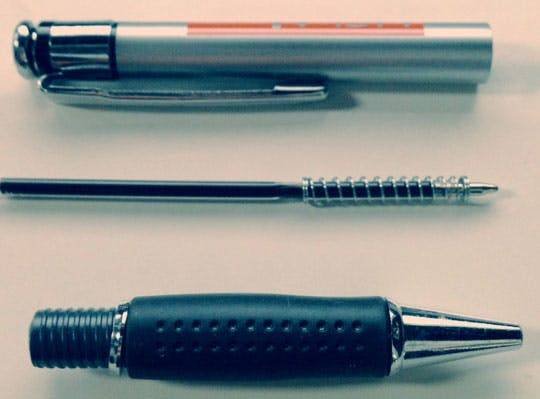
\includegraphics[width=.9\linewidth]{./pictures/pen-spring.jpg}
\end{center}
\end{column}
\end{columns}
\end{frame}

\begin{frame}[label={sec:org78b40b3}]{Mechanical Spring Types}
\begin{tabular}{cc}
    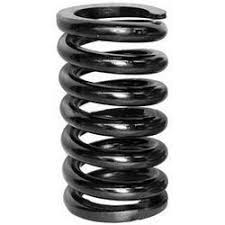
\includegraphics[width=0.45\textwidth]{pictures/helical-spring} &
    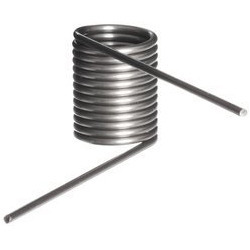
\includegraphics[width=0.45\textwidth]{pictures/torsion-spring} \\
    Helical Spring & Torsion Spring
\end{tabular}
\end{frame}

\begin{frame}[label={sec:orga484b4f}]{Mechanical Spring Types}
\begin{tabular}{cc}
  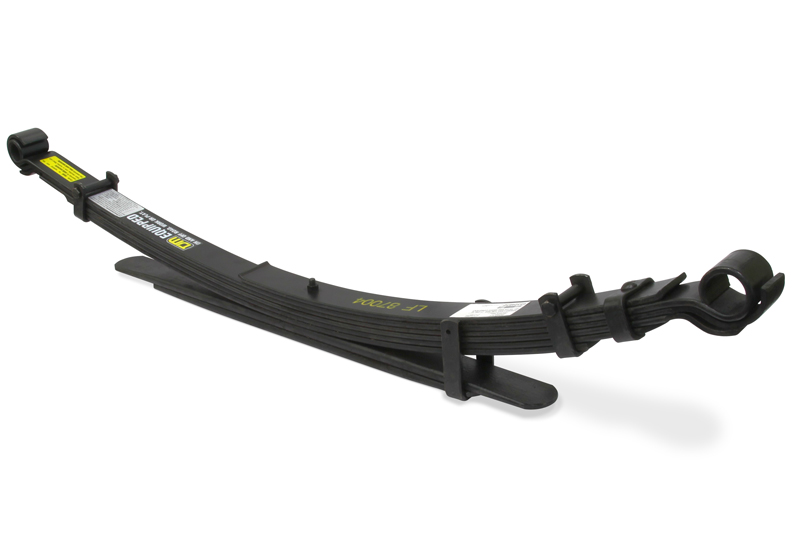
\includegraphics[width=0.45\textwidth]{pictures/leaf-spring} &
  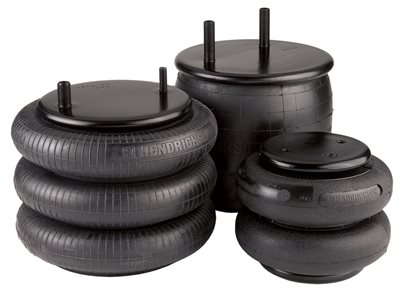
\includegraphics[width=0.45\textwidth]{pictures/air-spring} \\
  Leaf Spring & Air Spring
\end{tabular}
\end{frame}

\begin{frame}[label={sec:orgc355cb7}]{Automotive Applications}
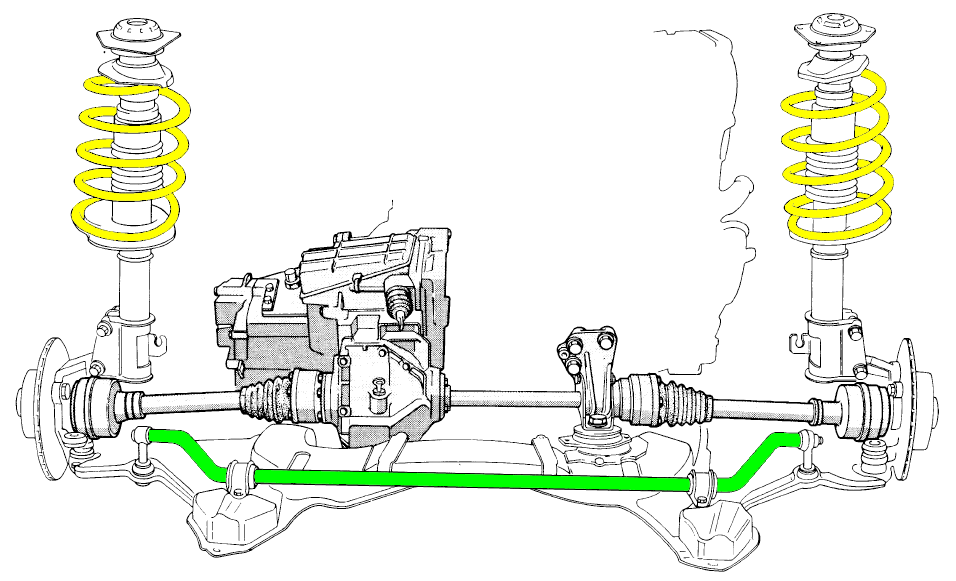
\includegraphics[width=0.9\textwidth]{pictures/car-suspension}
\end{frame}

\begin{frame}[label={sec:org7e8fb85}]{Automotive Applications}
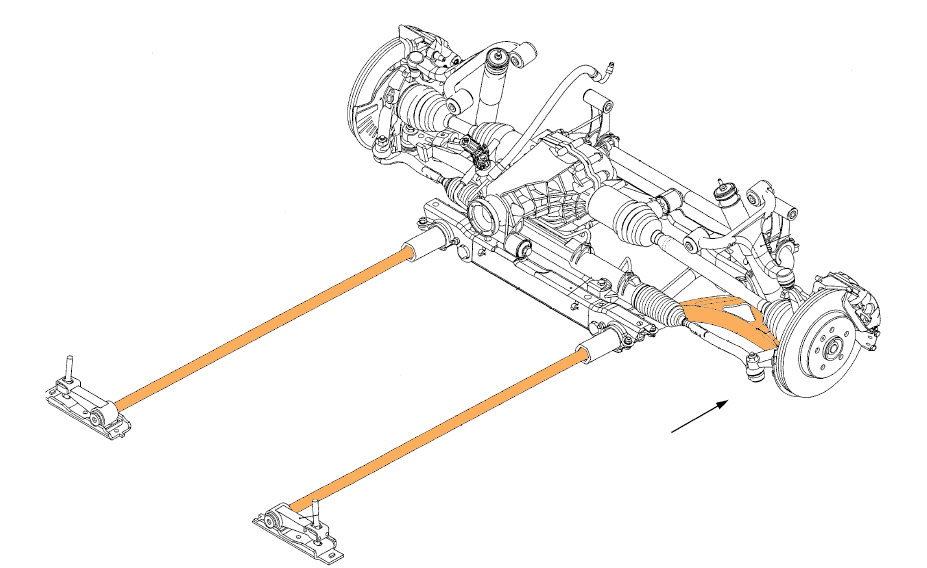
\includegraphics[width=0.9\textwidth]{pictures/front-suspension}
\end{frame}

\begin{frame}[label={sec:orgc1c6f62}]{Automotive Applications}
\centering
  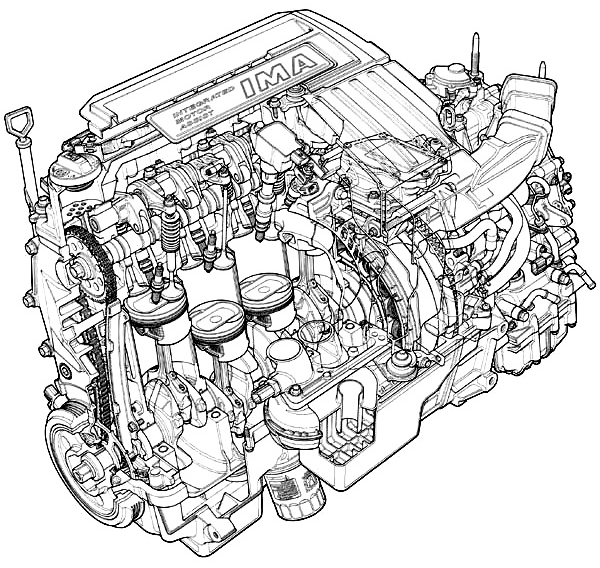
\includegraphics[width=0.7\textwidth]{pictures/engine}
\end{frame}

\begin{frame}[label={sec:org01e65cd}]{Main Focus: Helical Springs}
\centering
\begin{tabular}{cc}
  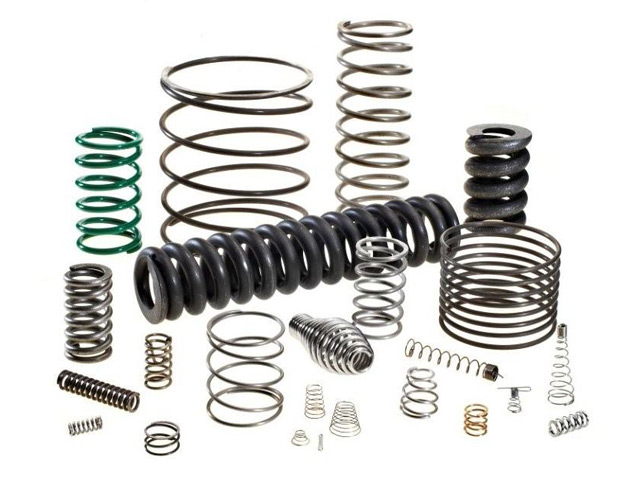
\includegraphics[width=0.45\textwidth]{pictures/compression-springs} &
  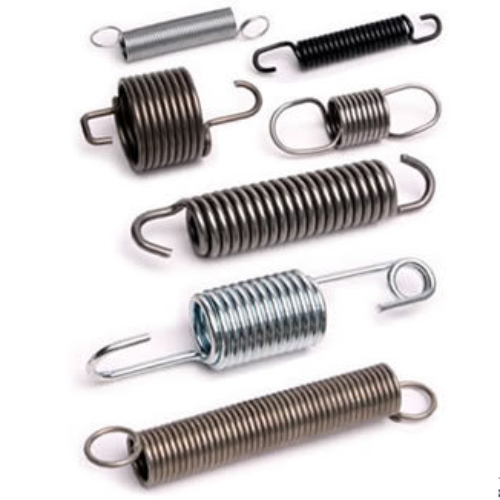
\includegraphics[width=0.45\textwidth]{pictures/tension-springs} \\
  Compression Springs & Tension Springs
\end{tabular}
\end{frame}

\section{Helical Compression Springs}
\label{sec:org2b510c1}

\begin{frame}[label={sec:orge20db30}]{Spring Lengths}
\centering
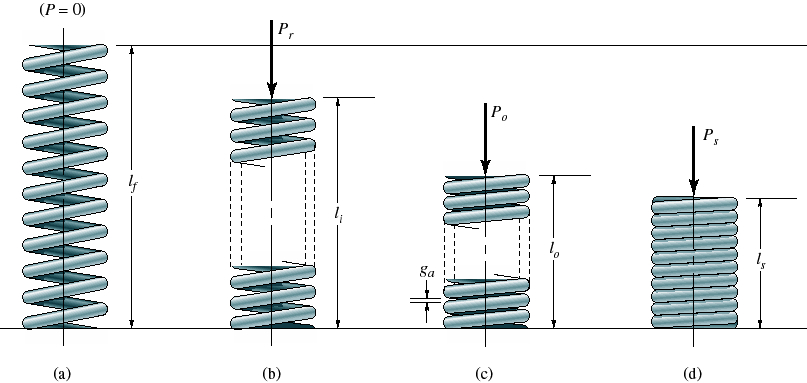
\includegraphics[width=\textwidth]{pictures/spring-lengths}
\end{frame}

\begin{frame}[label={sec:orga2ea3e1}]{Helical Spring Terminology}
\begin{columns}
\begin{column}{0.4\columnwidth}
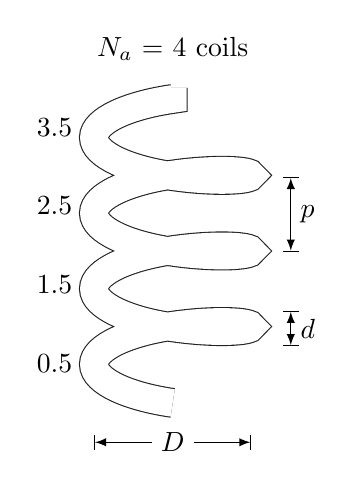
\begin{tikzpicture}[>=latex]
  \draw [decoration={aspect=0.25, segment length=0.96cm, amplitude=1cm, coil}, decorate, double, double distance=10pt, DarkGrey!20!Black] (0,0) node(A){} --++ (90:4) node(B){};
  \draw [|<->|] (A.center) ++ (-90:0.5) ++ (180:1) --++ (0:2) node[midway, fill=White]{$D$};
  \draw [|<->|] (A.center) ++ (0:1.5) ++ (90:0.72) --++ (90:0.45) node[midway, right]{$d$} node(C){};
  \draw [|<->|] (C.center) ++ (90:0.75) --++ (90:0.95) node[midway, right]{$p$};
  \node at (A.center) [xshift=-1.5cm, yshift=0.5cm] {0.5};
  \node at (A.center) [xshift=-1.5cm, yshift=1.5cm] {1.5};
  \node at (A.center) [xshift=-1.5cm, yshift=2.5cm] {2.5};
  \node at (A.center) [xshift=-1.5cm, yshift=3.5cm] {3.5};
  \node at (A.center) [xshift=0cm, yshift=4.5cm] {$N_a$ = 4 coils};
\end{tikzpicture}
\end{column}

\begin{column}{0.6\columnwidth}
\begin{itemize}
\item \(D\) = Coil Diameter
\item \(d\) = Wire Diameter
\item \(p\) = Pitch
\item \(N_a\) = Number of Active Coils
\end{itemize}
\end{column}
\end{columns}
\end{frame}

\begin{frame}[label={sec:org8b8b1c6}]{Compression Spring End Types}
\begin{center}
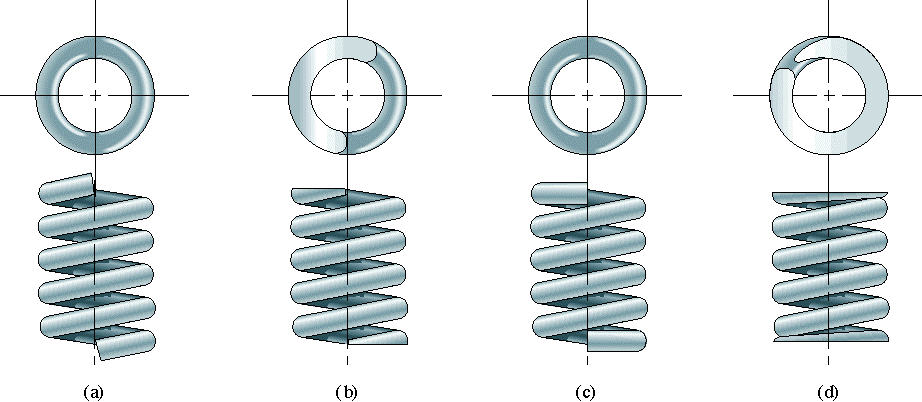
\includegraphics[width=.9\linewidth]{./pictures/end-types.png}
\end{center}

\scriptsize
\begin{tabular}{lllll}
  \toprule
  Term                       & Plain              & Plain and ground & Squared or closed & Squared and ground \\
  \midrule
  End coils, $N_e$ & 0                  & 1                & 2                 & 2                  \\
  Total coils, $N_t$& $N_a$             & $N_a + 1$        & $N_a + 2$         & $N_a + 2$           \\
  Free length, $l_f$         & $p N_a + d$        & $p(N_a+1)$        & $pN_a+3d$         & $pN_a+2d$           \\
  Solid length, $l_s$        & $d(N_{t}+1)$       & $dN_t$           & $d(N_t+1)$         & $dN_t$             \\
  pitch, $p$                 & $(l_f-d)/N_a$      & $l_f/(N_a+1)$     & $(l_f-3d)/N_a$    & $(l_f-2d)/N_a$      \\
  \bottomrule
\end{tabular}
\end{frame}

\begin{frame}[label={sec:org7287d60}]{Stress Analysis in Compression Springs}
\begin{center}
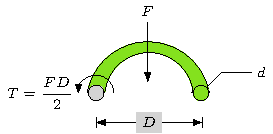
\includegraphics[width=.9\linewidth]{pictures/comp-spring-stress-analysis.pdf}
\end{center}

\vspace{0.5cm}
\normalsize
\begin{align*}
  \tau = \frac{Tr}{J} + \frac{F}{A} &= \frac{(FD/2)(d/2)}{\pi d^4 / 32} +
                                      \frac{F}{\pi d^2 / 4} \\
                                    &= \frac{8FD}{\pi d^3} + \frac{4F}{\pi d^2}
\end{align*}
\end{frame}

\begin{frame}[label={sec:org8aec31b}]{Stress in Helical Compression Springs}
\begin{itemize}
\item Combine answer to become
$$ \tau = K \frac{8FD}{\pi d^3} $$
\item where
$$ K = \frac{4C+2}{4C-3} $$
$$ C = \frac{D}{d} $$
\end{itemize}
\end{frame}

\begin{frame}[label={sec:orgb7e646f}]{Helical Spring Constant, \(k\)}
\begin{itemize}
\item Using energy method
$$ k = \frac{Gd^4}{8D^3N_a} = \frac{Gd}{8C^3N_a} $$
\end{itemize}
\end{frame}

\begin{frame}[label={sec:orge0d18a6}]{Material Strength}
\begin{itemize}
\item Material strength varies with wire diameter
$$ S_{ut} [MPa] = \frac{A [MPa \cdot mm^m]}{d[mm]^m} $$
\item Converting to SI units
$$ S_{ut} = \frac{A \cdot 10^6 \cdot 10^{-3m}}{d^m} $$
\item Allowable shear stress in spring material
$$ \tau_{allow} \approx 0.5 S_{ut} $$
\end{itemize}
\end{frame}

\begin{frame}[label={sec:orgda47365}]{Spring Material Properties}
\footnotesize
\begin{tabular}{ l c c c c c }
  \toprule
  Material & Diameter (mm) & G (GPa) & A (MPa-mm) & m & Relative Cost \\
  \midrule
  Music & 0.1 – 6.5 & 81.7 & 2211 & 0.145 & 2.6 \\
  \midrule
  OQ\&T & 0.5 – 12.7 & 77.2 & 1855 & 0.187 & 1.3 \\
  \midrule
  Hard-drawn & 0.7 – 12.7 & 79.3 & 1783 & 0.190 & 1.0 \\
  \midrule
  Chrome-vanadium & 0.8 – 11.1 & 77.2 & 2005 & 0.168 & 3.1 \\
  \midrule
  Chrome-silicon & 1.6 – 9.5 & 77.2 & 1974 & 0.108 & 4.0 \\
  \midrule
  \multirow{3}{2.2cm}{302 stainless steel} & 0.3 – 2.5 & \multirow{3}{1cm}{\centering 69} & 1867 & 0.148 & \multirow{3}{2cm}{\centering 7.6 – 11} \\
           & 2.5 – 5 & & 2065 & 0.263 & \\
           & 5 – 10 & & 2911 & 0.478 & \\
  \midrule
  \multirow{3}{2.2cm}{Phosphor-bronze} & 0.1 – 0.6 & \multirow{3}{1cm}{\centering 41} & 1000 & 0 & \multirow{3}{2cm}{\centering 8.0} \\
           & 0.6 – 2 & & 913 & 0.028 & \\
           & 2 – 7.5 & & 932 & 0.064 & \\
  \bottomrule
\end{tabular}
\end{frame}

\begin{frame}[label={sec:orgfad4fcc}]{Spring Material Specifications}
\small
\begin{tabular}{ l p{8cm}}
  \toprule
  Materials & \multicolumn{1}{c}{Descriptions}  \\
  \midrule
  Music & Excellent for small springs, repeated loadings \\
  \midrule
  OQ\&T* & Good for gen purpose. Not for shock or impact. \\
  \midrule
  Hard-drawn & Cheap. Really cheap. \\
  \midrule
  Chrome-vanadium & Excellent for high stress, fatigue, impact, and shock. \\
  \midrule
  Chrome-silicon & Excellent for high stress and shock. Good longevity. \\
  \bottomrule
\end{tabular}
\end{frame}

\begin{frame}[label={sec:orge81dcb8}]{Vibration Issue}
\begin{itemize}
\item To avoid resonance

\begin{gather*}
\omega_{\text{spring}} \geq (15 - 20)\omega_{\text{sys}} \\
\omega_{\text{spring}} = \left\{
  \begin{array}{ll}
    \dfrac{1}{2}\sqrt{\dfrac{k}{m}} & \text{fixed-fixed} \\
    \dfrac{1}{4}\sqrt{\dfrac{k}{m}} & \text{fixed-free}
  \end{array}
\right.
\end{gather*}

\begin{itemize}
\item where \(m\) is the spring mass
\end{itemize}
\end{itemize}
\end{frame}

\begin{frame}[label={sec:org22f100a}]{Spring Buckling}
\scriptsize
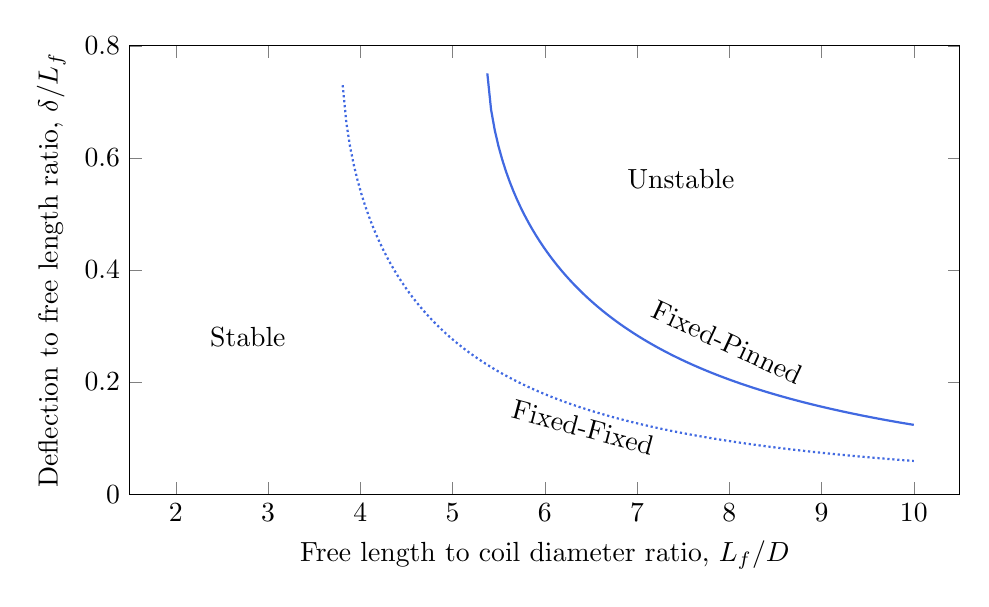
\begin{tikzpicture}
  \begin{axis}[
    height=0.6\textwidth,
    width=\textwidth,
    % axis background/.style={fill=SkyBlue!50},
    axis line style={->},
    % grid=both,
    % grid style={draw=Grey!10},
    xmin=1.5, xmax=10.5,
    xlabel={Free length to coil diameter ratio, $L_f / D$},
    ymin=0, ymax=0.8,
    ylabel={Deflection to free length ratio, $\delta / L_f$}]
    %% C1 = 0.79, C2 = 7.21

    \addplot [RoyalBlue,thick,domain=2:10,samples=200]{0.79*(1-sqrt(1-7.21/(0.5*\x)^2))} node[midway, xshift=4mm, yshift=3mm, black, rotate=-25]{Fixed-Pinned};
    \addplot [RoyalBlue,thick, densely dotted,domain=2:10,samples=200]{0.79*(1-sqrt(1-7.21/(0.707*\x)^2))} node[midway, xshift=-5mm, yshift=-1mm, black, rotate=-15]{Fixed-Fixed};
  \end{axis}
  \node at (7,4) {Unstable};
  \node at (1.5,2) {Stable};
\end{tikzpicture}
\end{frame}

\begin{frame}[label={sec:orgbc22b2c}]{Simple Buckling Rule of Thumb}
\begin{itemize}
\item General rule of thumb is max deflection should be less than 80$\backslash$% of range

$$ \frac{\delta_{\max}}{{{N_a}(p - d)}} = 0.8 $$
\end{itemize}
\end{frame}

\begin{frame}[label={sec:orgc574b46}]{Maximum Compressive Load}
\begin{itemize}
\item Maximum compressive load must not cause solid length
\begin{gather*}
  F_{\max}  < F_s \\
  F_s = F_{\max}(1 + \xi) \\
  \xi \geqslant 0.15
\end{gather*}
\end{itemize}
\end{frame}

\begin{frame}[label={sec:org6f462c2}]{Compressive Spring Design for Static Loading}
\begin{itemize}
\item Allowable compressive stress \(>\) stress at solid length
\end{itemize}

$$ \frac{\tau_{allow}}{N_s} = \frac{8KF_sD}{\pi d^3} $$
$$ K = \frac{4C+2}{4C-3} $$ 
$$ F_s = F_{\max}(1+\xi) $$

$$ \frac{\tau_{allow}}{N_s} = \frac{4C+2}{4C-3} \left[ \frac{8F_{\max}(1+\xi)C}{\pi d^2} \right] $$
\end{frame}

\begin{frame}[label={sec:orgaac5058}]{Solving for Spring Index \(C\)}
$$ \alpha = \frac{\tau_{allow}}{N_s} $$
$$ \beta = \frac{8F_{\max}(1+\xi)}{\pi d^2} $$

$$ C = \frac{2\alpha - \beta}{4\beta} + \sqrt{ \left( \frac{2\alpha - \beta}{4\beta} \right)^2 - \frac{3\alpha}{4\beta} } $$
\end{frame}

\begin{frame}[label={sec:org801a2ba}]{General Guidelines for Compressive Helical Springs}
$$ 4 \leqslant C \leqslant 12 $$
$$ 3 \leqslant N_a \leqslant 15 $$
$$ N_s \geqslant 1.2 $$
$$ \xi \geqslant 0.15 $$

\begin{itemize}
\item Minimize spring mass
\end{itemize}

$$ m = \frac{\rho \pi^2 d^2 N_t D}{4} $$
\end{frame}

\begin{frame}[label={sec:orge2f6088}]{Example: Car Suspension Springs}
\begin{enumerate}
\item Empty car (1200 kg) should stand 15 cm from the ground.
\item Fully loaded car (add 150 kg to the front seats and 200 kg to the rear seat) should stand 13 cm above the ground (front) and 12 cm above the ground (rear).

Design the front and rear suspension springs.

\centering
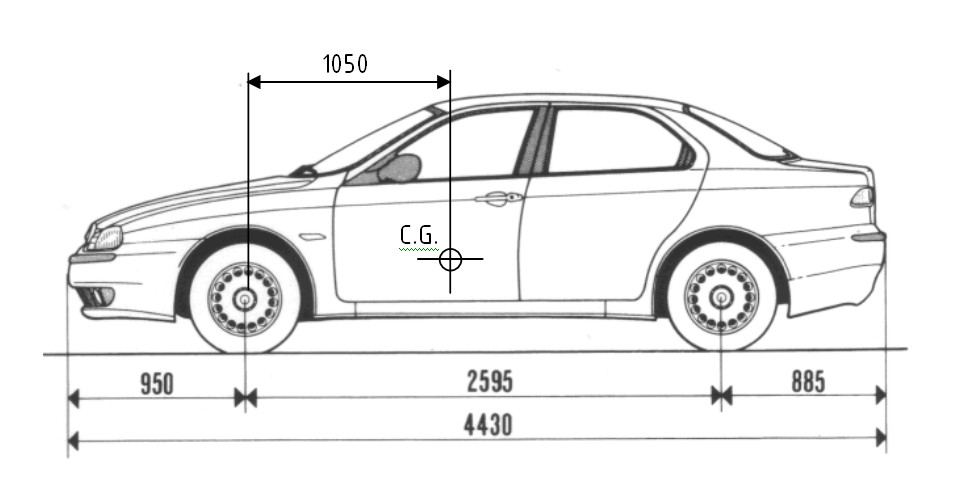
\includegraphics[width=0.7\textwidth]{pictures/car-example}
\end{enumerate}
\end{frame}

\begin{frame}[label={sec:org9e952de}]{Solution}
First, we need to find the maximum load in the front and rear suspension. Use static equilibrium. For the empty car
\begin{align*}
  2F_{r1}(2595) &= 12000(1050) \\
  F_{r1} &= 2428 \text{ N} \\
  2F_{f1} &= 12000 - 2(4856) = 7144 \\
  F_{f1} &= 3572 \text{ N}
\end{align*}
\end{frame}

\begin{frame}[label={sec:org76f0b23}]{Solution}
For the fully loaded car, the added front load goes at the c.g., while the read load goes in the middle of c.g. and rear wheel. The distance from the rear load to the rear wheel is
\begin{gather*}
  d_r = \frac{2595 - 1050}{2} = 772.5 \text{ mm}
\end{gather*}
The front and rear loads in the fully loaded car are
\begin{align*}
  2F_{f2}(2595) &= (12000 + 1500)(2595 - 1050) + 2000(772.5) \\
  F_{f2} &= 4316 \text{ N} \\
  2F_{r2} &= 12000 + 1500 + 2000 - 2(4316) \\
  F_{r2} &= 3434 \text{ N}
\end{align*}
\end{frame}

\begin{frame}[label={sec:org69892b3}]{Solution}
Setting \(N_s\) = 1.25 and \(\xi\) = 0.15, if we choose \(d\) = 15 mm for the front suspension, the spring index \(C\) can be calculated.
\begin{align*}
  \alpha  &= \frac{\tau_{allow}}{N_s} = \frac{0.5}{1.25}\frac{2005}{15^{0.168}} \times {10^6} = 509 \text{ MPa} \\ 
  \beta  &= \frac{8(1 + \xi )F_{\max}}{\pi d^2} = \frac{8(1 + 0.15)4316}{\pi {(15 \times 10^{ - 3})}^2} = 56.2 \text{ MPa}
\end{align*}
\begin{align*}
  C &= \frac{2\alpha  - \beta}{4\beta} + \sqrt {\left( \frac{2\alpha  - \beta}{4\beta} \right)^2 - \frac{3\alpha}{4\beta}}  \\ 
    & = \frac{2(509) - 56.2}{4(56.2)} + \sqrt {\left( \frac{2(509) - 56.2}{4(56.2)} \right)^2 - \frac{3(509)}{4(56.2)}}  \\ 
    &= 7.7 
\end{align*}
\end{frame}

\begin{frame}[label={sec:orga07777f}]{Solution}
We perform the same calculation for the rear springs. Pick \(d\) = 13 mm since the maximum force is slightly smaller than the front springs.
 \begin{align*}
   \alpha  &= \frac{{{\tau_{allow}}}}{{{N_s}}} = \frac{{0.5}}{{1.25}}\frac{{2005}}{{{{13}^{0.168}}}} \times {10^6} = 521 \text{ MPa} \\ 
  \beta  &= \frac{{8(1 + \xi ){F_{\max }}}}{{\pi {d^2}}} = \frac{{8(1 + 0.15)3434}}{{\pi {(13 \times 10^{ - 3})}^2}} = 59.5 \text{ MPa}
\end{align*}
\begin{align*}
  C &= \frac{{2\alpha  - \beta }}{{4\beta }} + \sqrt {{{\left( {\frac{{2\alpha  - \beta }}{{4\beta }}} \right)}^2} - \frac{{3\alpha }}{{4\beta }}}  \\ 
    & = \frac{{2(521) - 59.5}}{4(59.5)} + \sqrt {{{\left( {\frac{{2(521) - 59.5}}{{4(59.5)}}} \right)}^2} - \frac{{3(521)}}{{4(59.5)}}}  \\ 
    &= 7.4 
\end{align*}
\end{frame}

\begin{frame}[label={sec:org2f13c7a}]{Solution}
\(D\) of the front and rear springs can be easily calculated
\begin{align*}
  D_f &= Cd = 7.7(15) = 116 \text{ mm} \\
  D_r &= 7.4(13) = 96.2 \text{ mm}
\end{align*}
Spring constants is needed to determine the required number of active coils \(N_a\).
\begin{align*}
  k_f &= \frac{\Delta F}{\Delta x} = \frac{4316 - 3572}{0.02} \\
      &= 37200 \text{ N/m} \\
  k_r &= \frac{3434 - 2428}{0.03} \\
      &= 33533 \text{ N/m}
\end{align*}
\end{frame}

\begin{frame}[label={sec:orged25010}]{Solution}
Determine the \(N_a\)
\begin{align*}
  {N_{af}} &= \frac{{Gd}}{{8{C^3}k}} = \frac{{77.2 \times {{10}^9}(15 \times {{10}^{ - 3}})}}{{8({{7.7}^3})(37200)}} = 8.6 \\
  {N_{ar}} &= \frac{{Gd}}{{8{C^3}k}} = \frac{{77.2 \times {{10}^9}(13 \times {{10}^{ - 3}})}}{{8({{7.4}^3})(33533)}} = 9.3 \\
\end{align*}
\end{frame}

\begin{frame}[label={sec:org28d7abc}]{Solution}
Determine pitch \(p\), as a rule of thumb, max deflection should not exceed 80\% of the spring compression range, which is \(N_a(p - d)\). The max deflection of the front and rear springs are
\begin{align*}
  \delta_f &= \frac{F_{f2}}{k_f} = \frac{4316}{37200} \\
           &= 1.16 \times 10^{-1} \text{ m} \\
  \delta_r &= \frac{F_{r2}}{k_r} = \frac{3434}{33533} \\
           &= 1.02 \times 10^{-1} \text{ m}
\end{align*}
\end{frame}

\begin{frame}[label={sec:orgf8440da}]{Solution}
Finally, the pitches of the front and rear springs are

\[\frac{\delta }{{{N_a}(p - d)}} = 0.8\]

\begin{align*}
  {p_f} &= \frac{\delta_f}{0.8 N_{af}} + {d_f} \\ 
        &= \frac{{1.16 \times {{10}^{ - 1}}}}{{0.8(8.6)}} + 15 \times {10^{ - 3}} \\ 
        &= 3.19 \times 10^{-2} \text{ m} \\
  {p_r} &= \frac{\delta_r}{0.8N_{ar}} + d_r \\ 
        &= \frac{1.02 \times 10^{-1}}{0.8(9.3)} + 13 \times 10^{-3} \\ 
        &= 2.67 \times {10^{ - 2}} \text{ m}
\end{align*}
\end{frame}

\section{Helical Extension Springs\}}
\label{sec:orga507437}

\begin{frame}[label={sec:orgbaea788}]{Helical Extension Springs}
\begin{itemize}
\item Ends are typically made into hooks or loops
\end{itemize}


\centering
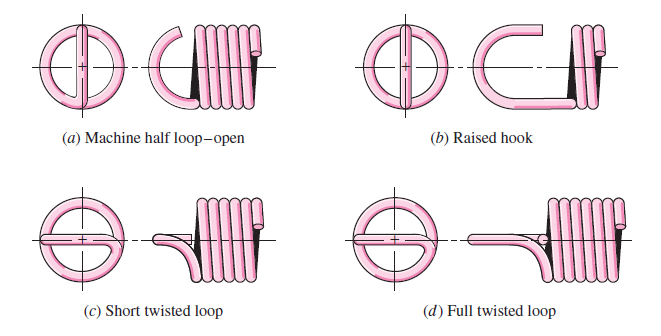
\includegraphics[width=0.9\textwidth]{pictures/extension-ends}
\end{frame}

\begin{frame}[label={sec:orgebaee61}]{Maximum Stress in Extension Springs}
\centering
\begin{tabular}[h]{cc}
  \multicolumn{2}{c}{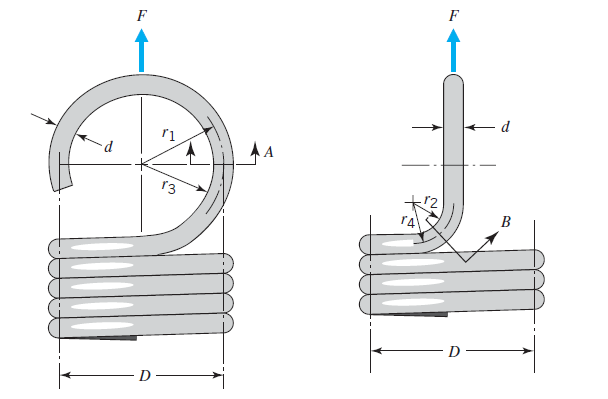
\includegraphics[width=0.7\textwidth]{pictures/max-stress-hooks}} \\
  $ \sigma_{\max} = \dfrac{16FD}{\pi d^3}\dfrac{r_1}{r_3} $ & $ \tau_{\max} = \dfrac{8FD}{\pi d^3}\dfrac{r_4}{r_2} $
\end{tabular}
\end{frame}

\begin{frame}[label={sec:org8c7e53b}]{Considerations for Extension Springs}
\begin{itemize}
\item No buckling or solid length
\item Only stress
\end{itemize}


$$ \sigma_{\max} \leqslant \frac{S_{ut}}{N_s} $$
$$ \tau_{\max} \leqslant \frac{\tau_{allow}}{N_s} $$
$$ 4 \leqslant C \leqslant 12 $$
$$ m = \frac{\rho \pi^2 d^2 N_t D}{4} $$
\end{frame}

\begin{frame}[label={sec:org05f4ac3}]{Chest Exercise Springs}
\begin{center}
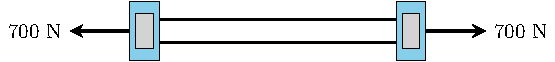
\includegraphics[width=.9\linewidth]{pictures/chest-exercise-example.pdf}
\end{center}

The maximum pulling force allowed is 700 N and the unstretched spring is 1 m long. Using a safety factor of 2,

\begin{itemize}
\item Determine the proper spring to be used.
\end{itemize}
\end{frame}

\begin{frame}[label={sec:orgea6a252}]{Solution}
The problem did not mention the maximum stretched length of the spring. However, this is a chest exercise machine and its reasonable maximum length should approximately be of a length of an average human reach, say 1.5 m. We can calculate the required spring stiffness.
\[k = \frac{\Delta F}{\Delta x} = \frac{350 - 0}{1.5 - 1} = 700 \text{ N/m} \]
\end{frame}

\begin{frame}[label={sec:orgf9514b8}]{Solution}
\begin{itemize}
\item Pick extension spring.
\item No requirements for shock load or corrosion resistance.
\item Pick the inexpensive \emph{hard-drawn} wire
\end{itemize}

Equations for required diameter is
\[\begin{gathered}
  \sigma _{\max } = \frac{16FD}{\pi d^3}\left( \frac{r_1}{r_3} \right) = \frac{16FC}{\pi d^2}\left( \frac{r_1}{r_3} \right) \hfill \\
  {\tau _{\max }} = \frac{{8FD}}{{\pi {d^3}}}\left( {\frac{{{r_4}}}{{{r_2}}}} \right) = \frac{{8FC}}{{\pi {d^2}}}\left( {\frac{{{r_4}}}{{{r_2}}}} \right) \hfill \\ 
\end{gathered} \]
\end{frame}

\begin{frame}[label={sec:orgab2b88c}]{Another Example?}
\begin{center}
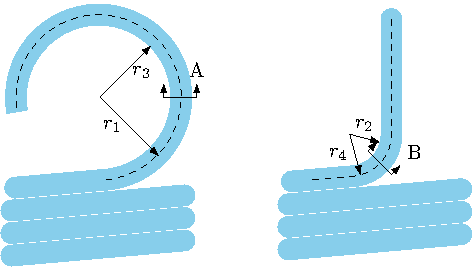
\includegraphics[width=.9\linewidth]{pictures/chest-exercise-end-coils.pdf}
\end{center}

According to the picture, \(r_1 = D / 2\), \(r_3 = (D - d) / 2\). Let us also assume that \(r_4 = D / 3\), which gives \(r_2 = D / 3 - d / 2\). For a relatively low stiffness spring, we will assume that the spring index \(C\) = 8, which allows us to solve for \(d\).
\end{frame}

\begin{frame}[label={sec:org67cffaf}]{Solution}
\begin{gather*}
  \sigma_{\max } = \frac{S_{ut}}{N_s} = \frac{16FC}{\pi d^2}\left( \frac{r_1}{r_3} \right) = \frac{16FC}{\pi d^2}\left( \frac{D}{D - d} \right) \\
  0.5\frac{A}{d^m} = \frac{16FC}{\pi d^2}\left( \frac{C}{C - 1} \right) \\ 
  0.5\frac{1783 \times {{10}^6} \times 10^{ - 3(0.190)}}{d^{0.190}} = \frac{16(350)(8)(8)}{\pi d^2(8 - 1)} \\
  \begin{aligned}
  &d^{2 - 0.190} = 6.79 \times {10^{ - 5}} \\ 
  &d = 4.98 \times {10^{ - 3}}\;{\text{m }} = 4.98\text{ mm}
  \end{aligned}
\end{gather*}
\end{frame}

\begin{frame}[label={sec:org43fcca2}]{Solution}
\begin{gather*}
  \tau_{\max } = \frac{\tau_{allow}}{N_s} = \frac{8FC}{\pi d^2}\left( \frac{r_4}{r_2} \right) = \frac{8FC}{\pi d^2}\left( \frac{D/3}{D/3 - d/2} \right) \\ 
  \frac{0.5}{2}\frac{A}{d^m} = \frac{8FC}{\pi d^2}\left( \frac{C/3}{C/3 - 1/2} \right) \\ 
  \frac{0.5}{2}\frac{1783 \times 10^6 \times 1^{ - 3(0.190)}}{d^{0.190}} = \frac{8(350)(8)(8/3)}{\pi d^2(8/3 - 1/2)} \\
  \begin{aligned}
  &d^{2 - 0.190} = 8.13 \times 10^{ - 5} \\ 
  &d = 5.50 \times 10^{ - 3}\text{ m} = 5.50 \text{ mm}
  \end{aligned}
\end{gather*}
\end{frame}

\begin{frame}[label={sec:orgcc11ffd}]{Solution}
\begin{itemize}
\item Choose \(d\) = 5.50 mm
\item Coil diameter \(D = Cd\) = 4.4 cm.

Finally, the number of required active coils is
\end{itemize}

\[N_a = \frac{Gd}{8C^3k} = \frac{79.3 \times 10^9(5.5 \times 10^{ - 3})}{8(8^3)(700)} = 152\text{ coils}\]
\end{frame}
\end{document}